\documentclass{article}
\usepackage[utf8]{inputenc}
\usepackage{amsmath}
\usepackage{amsfonts}
\usepackage{graphicx}

\title{Written Assignment Unit 1\\
Math 1201- College Algebra.
}
\author{Instructor - Casmir Onyeneke}
\date{September 2021}


\begin{document}

\maketitle

\section*{Question 1}
Find the domain of the function using the interval notation.
$${f(x) = \frac{\sqrt{x-6}}{\sqrt{x-4}}}$$
Here we have fractional equation that contains square root both in its numerator and denominator.\\
in order to find the domain of the function we have to resolve the domain of both in the numerator and denominator and then combine them.\\

For the numerator

$${\sqrt{x-6}}$$
Because it is a square root, the radicand can never be negative, therefore we equate it to ${\ge 0}$
$${x - 6 \ge 0}$$
Adding 6 to both sides
$${x\ge6}$$\\

For the denominator
$${\sqrt{x-4}}$$
Because it is a square root, which also happens to be a denominator in the expression, the radicand can never be negative or equal to zero. Therefore the radicand can only be greater than zero ${> 0}$
$${x-4>0}$$
Adding 4 to both sides.
$${x > 4}$$

On the number line any value between 4 and 6 excluding 6 will result in a numerator that has a negative radicand and this is not allowed, but if we take an input value of 6 and above, the radicands of both the numerator and the denominator are satisfied as they are both greater than zero.\\
Therefore the domain for this function in interval notation is  $$[6,\infty)$$




$${}$$


\section*{Question 2}
\textbf{Sketch a graph of a piecewise function and Write the domain in interval notation}\\
My functions are ${y = x^2 + 10  for  \{-2<x<2\}}$\\
and ${y = 2x+10 for \{1<x<10\}}$

\begin{equation*}
    f(x)=\begin{cases}
            y = x^2 + 10  \quad & \text{if}  \{-2<x<2\} \\
            y = 2x+10 \quad & \text{if} \{1<x<10\} \\
        \end{cases}
    \end{equation*}
The domain for the first equation is ${(-2,2)}$\\
The domain for the second equation is  ${(1,10)}$\\
The final domain in interval notation is ${(-2,2)\cup(1,10)}$

The graph is shown below

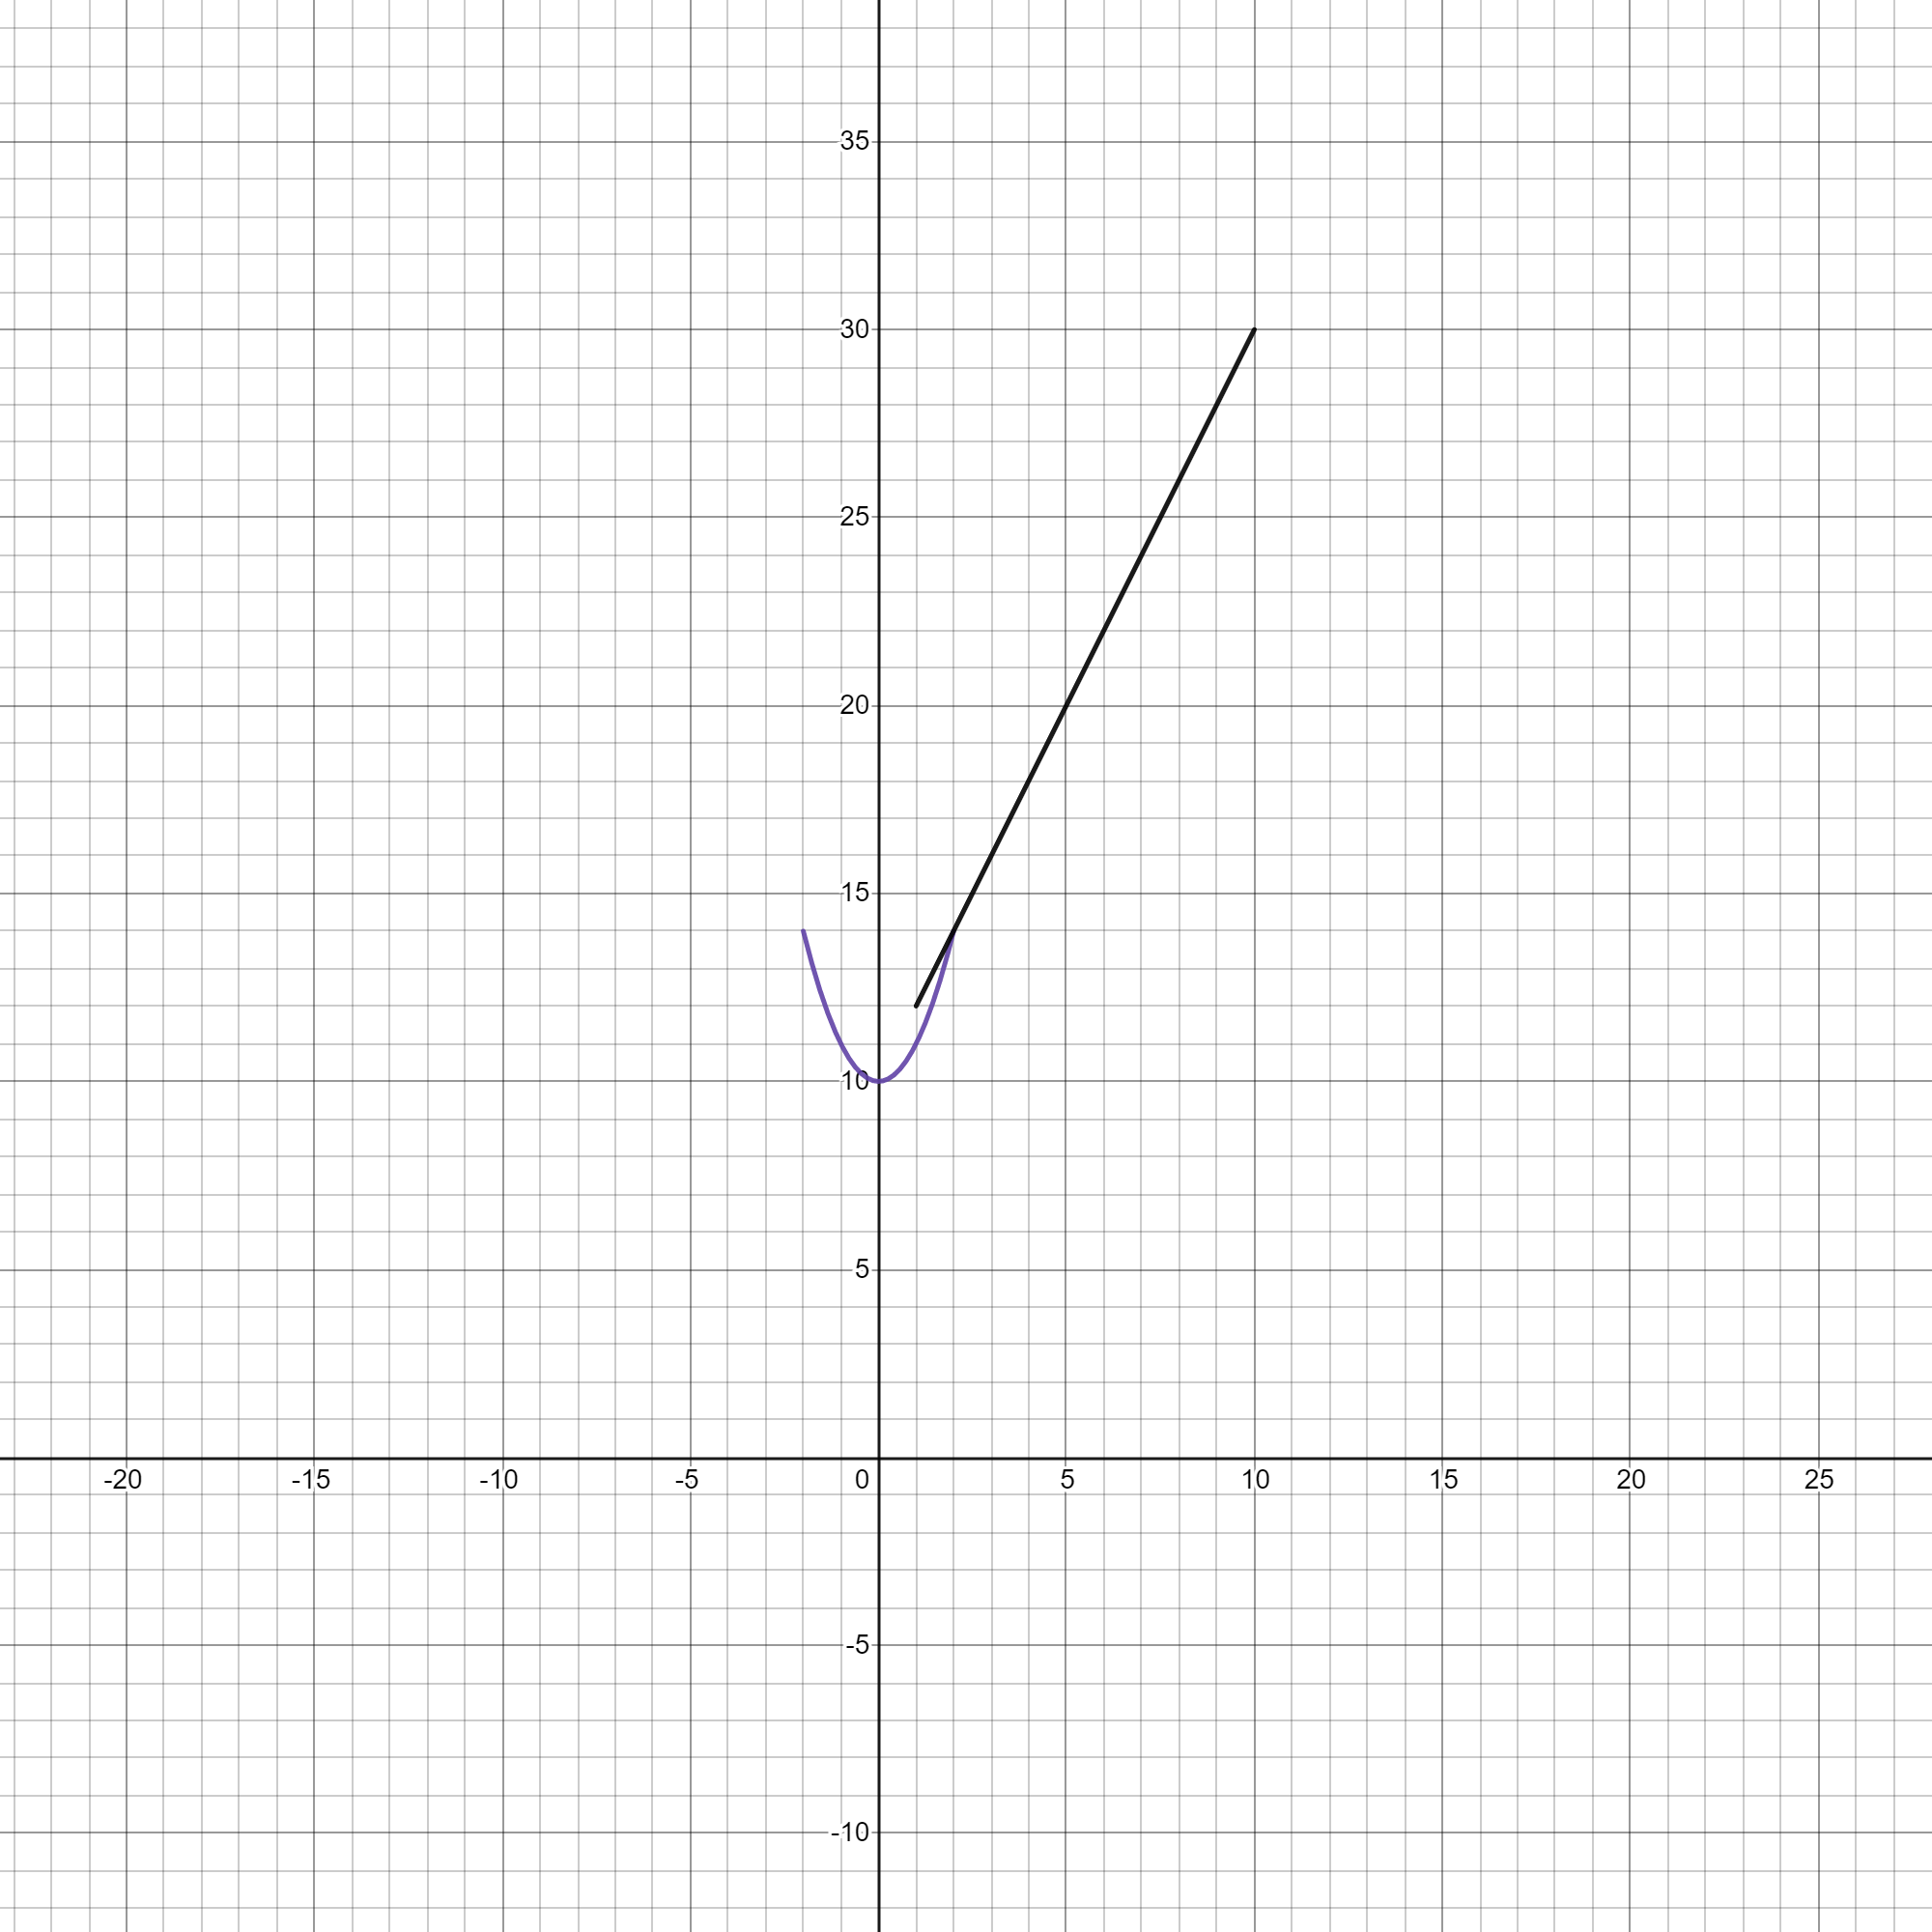
\includegraphics[scale = 0.1]{WOne_WA-Q2}

\section*{Question 3}
The cost in dollars of making ${x}$ items is given by the function 
$${C(x) = 10x + 500}$$
\begin{itemize}
    \item \textbf{A.}  The fixed cost is determined when zero items are produced. Find the fixed cost for this item.
    
    x as a  variable determines the number of items made.\\
    Therefore to find the fixed cost we have to evaluate the function ${C(x)}$
\\\\
    for x = 0
    $${C(0) = 10(0) + 500}$$
    $${C(0) = 0 + 500}$$
    $${C(0) = 500}$$
    Therfore the fixed cost for Zero items produced is \$500
    

    \item \textbf{B.}  What is the cost of making 25 items?\\
    For the cost of making 25 items, ${x = 25}$
    
    $${C(25) = 10(25) + 500}$$
    $${C(25) = 250 + 500}$$
    $${C(25) = 750}$$
    Therefore the cost of making 25 items is \$750.
    
    \item \textbf{C.}  Suppose the maximum cost allowed is \$1500. What are the domain and range of the cost function, C(x)?\\
    if the maximum cost is \$1500, then the function of C(x) can be expressed as
    $${10x + 500 \le 1500}$$
    Now solving for x
    $${10x + 500 \le 1500}$$
    subtracting 500 from both sides
    $${10x \le 1500 - 500}$$
    $${10x \le 1000}$$
    dividing both sides by 10
    $${ x \le \frac{1000}{10}}$$
    $${ x \le 100}$$

    What this means is that if the maximum price is \$1500, the most items we would be able to make is 100.

    So In summary \$1500, the domain is [0, 100] or ${0 \le x \le 100}$

    The range on the other hand is [500, 1500] or ${ \$500 \le y \le \$1500}$ 


\end{itemize}





\section*{REFERENCES}
Abramson, J. (2017). \textit{Algebra and trigonometry}. OpenStax, TX: Rice University. Retrieved
from https://openstax.org/details/books/algebra-and-trigonometry

\end{document}
